\documentclass[sectiontocframe default=off, aspectratio=169]{beamer}

%%%%%%%%%%%%%%%%%%%    PACKAGES    %%%%%%%%%%%%%%%%%%%
%% Font
\usepackage{fontspec}
	\setmainfont{TexGyrePagella}

\usepackage{fontawesome5}

\usepackage{unicode-math}
	\setmathfont{TexGyrePagella-math}

%% Languages
\usepackage{polyglossia}
	\setdefaultlanguage[variant=british]{english}

%% Bibliography
\usepackage[style = authoryear, maxnames = 1]{biblatex}
\addbibresource{./centralised_bibliography/references.bib}

%% Maths
\usepackage{amsmath}
\usepackage{luacode}
\usepackage{cancel}

%% Colours
\usepackage{xcolor}
\definecolor{egyptRed}{HTML}{DD5129}
\definecolor{egyptBlue}{HTML}{0F7BA2}
\definecolor{egyptGreen}{HTML}{43B284}
\definecolor{egyptYellow}{HTML}{FAB255}

\definecolor{blueGrey}{HTML}{EEF2F6}

%% Graphics
\usepackage{tikz}
\usepackage{pgfplots}
	\pgfplotsset{compat=1.18}
	\pgfplotsset{set layers}

% Tikz libraries
\usetikzlibrary{overlay-beamer-styles}
\usetikzlibrary{positioning}
\usetikzlibrary{arrows.meta}
\usetikzlibrary{calc}

% Pgfplots libraries
\usepgfplotslibrary{fillbetween}

%% Tikz commands
% Styles
\tikzset{arrow/.style = {> = {Latex[length = 1.2mm]}}}

% Database node style
\makeatletter
	\tikzset{
		database/.style={
		path picture={
		\draw[fill = #1] (0, 1.5*\database@segmentheight) circle [x radius=\database@radius,
		y radius=\database@aspectratio*\database@radius];
		\draw (-\database@radius, 0.5*\database@segmentheight) arc [start angle=180,end angle=360,x radius=\database@radius,
		y radius=\database@aspectratio*\database@radius];
		\draw (-\database@radius,-0.5*\database@segmentheight) arc [start angle=180,end angle=360,x radius=\database@radius,
		y radius=\database@aspectratio*\database@radius];
		\draw (-\database@radius,1.5*\database@segmentheight) -- ++(0,-3*\database@segmentheight) arc [start angle=180,end angle=360,
		x radius=\database@radius, y radius=\database@aspectratio*\database@radius] -- ++(0,3*\database@segmentheight);
		},
		minimum width=2*\database@radius + \pgflinewidth,
		minimum height=3*\database@segmentheight + 2*\database@aspectratio*\database@radius + \pgflinewidth,
		},
		database segment height/.store in=\database@segmentheight,
		database radius/.store in=\database@radius,
		database aspect ratio/.store in=\database@aspectratio,
		database segment height=0.1cm,
		database radius=0.25cm,
		database aspect ratio=0.35,
	}
\makeatother

%% Others
\usepackage{siunitx}

%%%%%%%%%%%%%%%%%%    PARAMETERS    %%%%%%%%%%%%%%%%%%
%% Theme
\usetheme{gotham}

%% Remove footer
\defbeamertemplate{frame footer}{default/emptyFoot}{}
\gothamset{footer template = emptyFoot}

%% Add logo IGN
\renewcommand{\gothamInstituteLogoSquare}[1][4 ex]{\includegraphics[height = #1]{./figures/IGN_logo.pdf}}
\renewcommand{\gothamtitlepagelogo}{\hspace{5cm}\includegraphics[height = 1.5cm]{./figures/IGN_logo.pdf}}

%----------------------------------------------------------------------------------------
%	PAGE TITLE
%----------------------------------------------------------------------------------------
\title{Taper and total aerial volumes}
\date{\today}
\author{Florence Gohon and Amaël Le Squin}
\institute{Institut National de l'information géographique et forestière}

%----------------------------------------------------------------------------------------
%	NEW COMMANDS
%----------------------------------------------------------------------------------------
\newcommand{\Fbft}{F_{\text{BFT}}}

\newcommand{\fnew}{f_{\text{new}}}
\newcommand{\hdec}{h_{\text{dec}}}

\newcommand{\Vtot}{V_{\text{tot}}}
\newcommand{\Vbft}{V_{\text{bole}}}
\newcommand{\Vcrn}{V_{\text{crown}}}

\newcommand{\Sigmabf}{\symbfup{\Sigma}}

\DeclareMathOperator{\MVN}{MVN}

%%%% Start document
\begin{document}

\maketitle

\section{Taper volume}

\begin{frame}{Single-variable and three-variable models}
	In tree sample\ldots{}
	\begin{itemize}
		\item trees \( j \), where \( c \), \( h \), \( \hdec \) are measured
		\[
			\Vbft(j) = f_{III}(c, h, \hdec)
		\]
		\item \emph{simplified} or \emph{remeasured} trees \( i \), where \( c \) is measured
		\[
			\cancel{ \Vbft(i) = \Vbft(j) }
			\to
			\cancel{ \Vbft(i) = \Vbft(j) \frac{c(i)}{c(j)} }
			\to
			\Vbft(i) = \Vbft(j) \frac{f_{I}(c(i))}{f_{I}(c(j))}
		\]
	\end{itemize}
\end{frame}

\begin{frame}{What we keep}
	\begin{itemize}
		\item Data sets source
		\item Linear models
		\item Transformations
	\end{itemize}

\[
	\left\{
	\begin{aligned}
		\Vbft &= \frac{c^2 h}{4 \pi \left( 1 - \frac{1{,}3}{h} \right)^2} \fnew \\
		\fnew &= f_{III}(c, h, \hdec)
	\end{aligned}
	\right.
\]
\bigskip
\[
	\ln(\Vbft) = f_{I}\big( \ln(c) \big)
\]
\end{frame}

\begin{frame}{What we change}
	\begin{itemize}
		\item Explanatory variables
		\begin{itemize}
			\item \(\hdec\) turns into \(\hdec'\)
			\item variables are shared by every species
			\item \(f(g)\) is dropped
		\end{itemize}
		\item Parameters
		\begin{itemize}
			\item the three-variable model is no longer cut-specific 
		\end{itemize}
		\begin{align*}
			\fnew &= \alpha + \beta c + \gamma \frac{\sqrt{c}}{\hdec'} + \delta \frac{\sqrt{\hdec'}}{c^2 h} + \eta \left( 1 - \frac{\hdec'}{h} \right) \\
			V_{\text{bole}, I} &= \mathrm{e}^{\alpha + \beta \ln(c) + \gamma \ln(c)^2 + \frac{\sigma^2}{2}}
		\end{align*}
	\end{itemize}
\end{frame}

\begin{frame}{Performances similar to current models}
	\begin{center}
		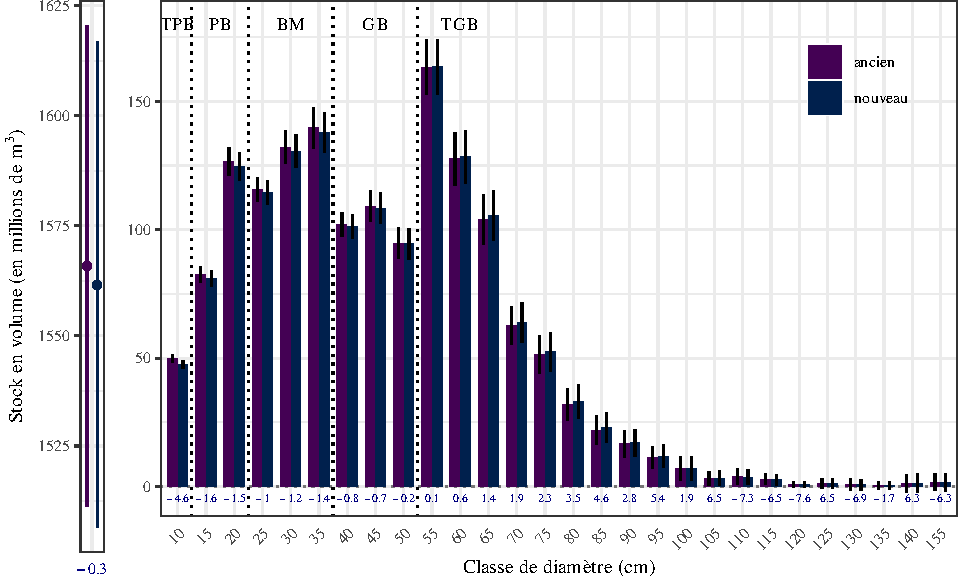
\includegraphics[scale = 0.7]{./figures/estimate_vbole_bygirth.pdf}
	\end{center}
\end{frame}

\section{Total aerial volume}
%%%% Tree frame
\begin{frame}{A tree in Emerge data}
	\begin{center}
		\begin{tikzpicture}
			\node[inner sep = 0pt] (tree) at (0, 0) {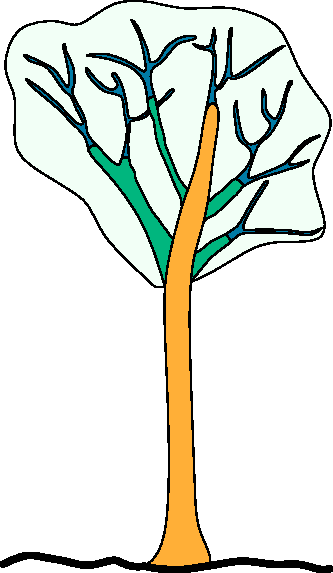
\includegraphics[scale = 0.65]{./pictures/ign_tree.pdf}};
			\matrix[anchor = north west, right = 0.8cm of tree] (legend)  at ([yshift=-1cm]tree.north east) {
				\node [draw, shape = rectangle, fill = egyptYellow, label = right:{Bole volume}] {}; \\
				\node [draw, shape = rectangle, fill = egyptGreen, label = right:{Large branches}] {}; \\
				\node [draw, shape = rectangle, fill = egyptBlue, label = right:{Small branches}] {}; \\
			};
		\end{tikzpicture}
	\end{center}
\end{frame}

%%%% 3 options to model
\begin{frame}{Three paths}
	\begin{center}
		\begin{enumerate}
			\item Bole volume (Florence) and independent crown model
			\item Multivariate model for both bole and crown volumes
			\item Model on the ratio between bole and total volumes
		\end{enumerate}
	\end{center}
\end{frame}

%%%% Option 1 --- results
\begin{frame}{Independent crown model -- 1}
	\begin{columns}
		\begin{column}{0.5\textwidth}
			\begin{center}
				\begin{tikzpicture}
\begin{axis}[
	xlabel={\( \Vbft \) (pred)},
	ylabel={\( \Vbft \) (obs)},
	tick label style={font=\small},
	label style={font=\small},
	width=6.5cm,
	height=6.5cm,
	axis on top,
	axis lines=left,
	tick align=outside,
	legend style={
		draw=none,
		fill=none,
		font=\small,
		at={(0, -0.3)},
		anchor=north west,
		/tikz/inner sep=1pt
	},
	% legend cell align=left,
	legend columns = 4,
	% xtick={-1,-0.5,0,0.5,1},
	% xticklabels={-1,-0.5,0,0.5,1},
	% ytick={0,0.5,1,.5},
	% yticklabels={0,0.5,1,.5},
	colormap = {egypt}{
		HTML = (DD5129)
		HTML = (0F7BA2)
		HTML = (43B284)
		HTML = (FAB255)
	}
]
\addlegendimage{only marks,mark=*,mark size=1.5pt,fill=egyptRed,draw=egyptRed},
\addlegendentry{Small},
\addlegendimage{only marks,mark=*,mark size=1.5pt,fill=egyptBlue,draw=egyptBlue},
\addlegendentry{Median},
\addlegendimage{only marks,mark=*,mark size=1.5pt,fill=egyptGreen,draw=egyptGreen},
\addlegendentry{Tall},
\addlegendimage{only marks,mark=*,mark size=1.5pt,fill=egyptYellow,draw=egyptYellow},
\addlegendentry{Very tall},
\addplot[
	scatter,
	only marks,
	mark=*,
	mark size=.75pt,
	point meta = explicit,
	scatter/use mapped color={
		fill=mapped color,
		draw=mapped color
	},
] table[
	x=bole_volume_m3_gohon,
	y=bole_volume_m3,
	meta = class,
	col sep=comma
] {inra_dec.csv};

\addplot[domain = 0:7, mark = none, thick] {x};

\end{axis}
\end{tikzpicture}
			\end{center}
		\end{column}
		%
		\begin{column}{0.5\textwidth}
			\begin{center}
				\begin{tikzpicture}
\begin{axis}[
	xlabel={\( \Vcrn \) (pred)},
	ylabel={\( \Vcrn \) (obs)},
	tick label style={font=\small},
	label style={font=\small},
	width=6.5cm,
	height=6.5cm,
	axis on top,
	axis lines=left,
	tick align=outside,
	legend style={
		draw=none,
		fill=none,
		font=\small,
		at={(0, -0.3)},
		anchor=north west,
		/tikz/inner sep=1pt
	},
	% legend cell align=left,
	legend columns = 4,
	% xtick={-1,-0.5,0,0.5,1},
	% xticklabels={-1,-0.5,0,0.5,1},
	% ytick={0,0.5,1,.5},
	% yticklabels={0,0.5,1,.5},
	colormap = {egypt}{
		HTML = (DD5129)
		HTML = (0F7BA2)
		HTML = (43B284)
		HTML = (FAB255)
	}
]
\addlegendimage{only marks,mark=*,mark size=1.5pt,fill=egyptRed,draw=egyptRed},
\addlegendentry{Small},
\addlegendimage{only marks,mark=*,mark size=1.5pt,fill=egyptBlue,draw=egyptBlue},
\addlegendentry{Median},
\addlegendimage{only marks,mark=*,mark size=1.5pt,fill=egyptGreen,draw=egyptGreen},
\addlegendentry{Tall},
\addlegendimage{only marks,mark=*,mark size=1.5pt,fill=egyptYellow,draw=egyptYellow},
\addlegendentry{Very tall},
\addplot[
	scatter,
	only marks,
	mark=*,
	mark size=.75pt,
	point meta = explicit,
	scatter/use mapped color={
		fill=mapped color,
		draw=mapped color
	},
] table[
	x=pred_crown_volume,
	y=crown_volume_m3,
	meta = class,
	col sep=comma
] {inra_dec.csv};

\addplot[domain = 0:4, mark = none, thick] {x};

\end{axis}
\end{tikzpicture}
			\end{center}
		\end{column}
	\end{columns}
\end{frame}

\begin{frame}{Independent crown model -- 2}
	\begin{center}
		\begin{tikzpicture}
\begin{axis}[
	xlabel={\( \Vcrn \) (pred)},
	ylabel={\( \Vcrn \) (obs)},
	tick label style={font=\small},
	label style={font=\small},
	width=7cm,
	height=7cm,
	axis on top,
	axis lines=left,
	tick align=outside,
	legend style={
		draw=none,
		fill=none,
		font=\small
	},
	legend cell align=left,
	legend pos = outer north east,
	% xtick={-1,-0.5,0,0.5,1},
	% xticklabels={-1,-0.5,0,0.5,1},
	% ytick={0,0.5,1,.5},
	% yticklabels={0,0.5,1,.5},
	colormap = {egypt}{
		HTML = (DD5129)
		HTML = (0F7BA2)
		HTML = (43B284)
		HTML = (FAB255)
	}
]
\addlegendimage{only marks,mark=*,mark size=1.5pt,fill=egyptRed,draw=egyptRed},
\addlegendentry{Small},
\addlegendimage{only marks,mark=*,mark size=1.5pt,fill=egyptBlue,draw=egyptBlue},
\addlegendentry{Median},
\addlegendimage{only marks,mark=*,mark size=1.5pt,fill=egyptGreen,draw=egyptGreen},
\addlegendentry{Tall},
\addlegendimage{only marks,mark=*,mark size=1.5pt,fill=egyptYellow,draw=egyptYellow},
\addlegendentry{Very tall},
\addplot[
	scatter,
	only marks,
	mark=*,
	mark size=.75pt,
	point meta = explicit,
	scatter/use mapped color={
		fill=mapped color,
		draw=mapped color
	},
] table[
	x=pred_total_volume,
	y=total_volume_m3,
	meta = class,
	col sep=comma
] {inra_dec.csv};

\addplot[domain = 0:8, mark = none, thick] {x};

\end{axis}
\end{tikzpicture}
	\end{center}
\end{frame}

%%%% Option 2 --- results
\begin{frame}{Multivariate model -- 1}
	\begin{columns}
		\begin{column}{0.5\textwidth}
			\begin{center}
				\begin{tikzpicture}
\begin{axis}[
	view={45}{55},
	grid=major,
	xlabel={\( \Vbft \)},
	ylabel={\( \Vcrn \)},
	zlabel={},
	xtick=\empty,
	ytick=\empty,
	ztick=\empty,
	width = 12cm,
	height = 12cm,
	domain = -5:5,
	y domain = -5:5,
	samples=40,
	zmin=0,
	zmax=0.4,
	axis lines=center,
	enlargelimits=0.1,
	every axis plot/.append style={line join=round},
	hide z axis=false,
	axis on top,
]

% ----------------------------------------------------------
% Parameters (mean, covariance)
% ----------------------------------------------------------
\pgfmathsetmacro{\mux}{0}
\pgfmathsetmacro{\muy}{0}
\pgfmathsetmacro{\sigx}{1}
\pgfmathsetmacro{\sigy}{sqrt(2)}
\pgfmathsetmacro{\rho}{0.6}

% ----------------------------------------------------------
% Random samples from MVN (Lua)
% ----------------------------------------------------------
\begin{luacode*}
math.randomseed(1234)
local N = 2000
local rho = 0.6
local sigx = 1.0
local sigy = math.sqrt(2)
local L11 = sigx
local L21 = rho * sigy
local L22 = sigy * math.sqrt(1 - rho^2)
tex.print("\\addplot3[only marks,mark=*,mark size=0.4pt,color=black,opacity=0.5]")
tex.print("table[row sep=crcr]{%")
for i=1,N do
	local z1 = math.sqrt(-2*math.log(math.random()))*math.cos(2*math.pi*math.random())
	local z2 = math.sqrt(-2*math.log(math.random()))*math.sin(2*math.pi*math.random())
	local x = L11*z1
	local y = L21*z1 + L22*z2
	tex.print(string.format("%.4f %.4f 0\\\\", x, y))
end
tex.print("};")
\end{luacode*}

% ----------------------------------------------------------
% Sigma ellipses (1σ, 2σ, 3σ)
% ----------------------------------------------------------
\foreach \k in {1,2,3}{
	\addplot3[domain=0:360,smooth,variable=\t,thick,green!60!black]
		({\k*(\sigx*cos(\t)+\rho*\sigy*sin(\t))}, {\k*(\sigy*sin(\t))}, {0.001});
}

% ----------------------------------------------------------
% 1D marginal PDFs (walls)
% ----------------------------------------------------------
\addplot3[
	domain=-5:5,
	samples=100,
	thick,
	color=blue
]
({x},{0},{1/(sqrt(2*pi)*\sigx)*exp(-0.5*(x/\sigx)^2)});

\addplot3[
	domain=-5:5,
	samples=100,
	thick,
	color=red
]
({-0},{x},{1/(sqrt(2*pi)*\sigy)*exp(-0.5*(x/\sigy)^2)});

\end{axis}
\end{tikzpicture}
			\end{center}
		\end{column}
		%
		\begin{column}{0.5\textwidth}
			\[
				\begin{pmatrix}
					\log(\Vbft) \\
					\log(\Vcrn)
				\end{pmatrix}
				\sim
				\MVN\left\{ \begin{pmatrix}
					f(c, \, h; \symbfup{\theta}) \\
					g(c, \, h; \symbfup{\theta}) \\
				\end{pmatrix}, \Sigmabf \right\}
			\]
		\end{column}
	\end{columns}
\end{frame}

\begin{frame}{Multivariate model -- 2}
	\begin{columns}
		\begin{column}{0.5\textwidth}
			\begin{center}
				\begin{tikzpicture}
\begin{axis}[
	xlabel={\( \Vtot \) (pred)},
	ylabel={\( \Vtot \) (obs)},
	tick label style={font=\small},
	label style={font=\small},
	width=6.5cm,
	height=6.5cm,
	axis on top,
	axis lines=left,
	tick align=outside,
	legend style={
		draw=none,
		fill=none,
		font=\small,
		at={(0, -0.3)},
		anchor=north west,
		/tikz/inner sep=1pt
	},
	legend columns = 4,
	colormap = {egypt}{
		HTML = (DD5129)
		HTML = (0F7BA2)
		HTML = (43B284)
		HTML = (FAB255)
	}
]
\addlegendimage{only marks,mark=*,mark size=1.5pt,fill=egyptRed,draw=egyptRed},
\addlegendentry{Small},
\addlegendimage{only marks,mark=*,mark size=1.5pt,fill=egyptBlue,draw=egyptBlue},
\addlegendentry{Median},
\addlegendimage{only marks,mark=*,mark size=1.5pt,fill=egyptGreen,draw=egyptGreen},
\addlegendentry{Tall},
\addlegendimage{only marks,mark=*,mark size=1.5pt,fill=egyptYellow,draw=egyptYellow},
\addlegendentry{Very tall},
\addplot[
	scatter,
	only marks,
	mark=*,
	mark size=.75pt,
	point meta = explicit,
	scatter/use mapped color={
		fill=mapped color,
		draw=mapped color
	},
] table[
	x=pred,
	y=obs,
	meta = class,
	col sep=comma
] {pred_tot.csv};

\addplot[domain = 0:8, mark = none, thick] {x};

\end{axis}
\end{tikzpicture}
			\end{center}
		\end{column}
		%
		\begin{column}{0.5\textwidth}
			\begin{center}
				\begin{tikzpicture}
\begin{axis}[
	xlabel={Circumference (RT)},
	ylabel={Residuals (RT)},
	tick label style={font=\small},
	label style={font=\small},
	xtick={0,0.25,0.5,0.75,1},
	xticklabels={0,0.25,0.5,0.75,1},
	ytick={0,0.25,0.5,0.75,1},
	yticklabels={0,0.25,0.5,0.75,1},
	width=6.5cm,
	height=6.5cm,
	tick align=outside,
	tick label style={font=\small},
	label style={font=\small},
	colormap = {egypt}{
		HTML = (DD5129)
		HTML = (0F7BA2)
		HTML = (43B284)
		HTML = (FAB255)
	}
]

%% Plot residuals
\addplot[
	scatter,
	only marks,
	mark=*,
	mark size=.75pt,
	point meta = explicit,
	scatter/use mapped color={
		fill=mapped color,
		draw=mapped color
	},
] table[
	x=circumference_rt,
	y=residuals,
	meta = class,
	col sep=comma
] {residuals.csv};

%% Quantile 25 and plygon
\addplot[name path=lower, draw=none] table[
	x=circumference_rt,
	y expr=\thisrow{q25} - \thisrow{err25},
	col sep=comma
]{residuals.csv};

\addplot[name path=upper, draw=none] table[
	x=circumference_rt, 
	y expr=\thisrow{q25} + \thisrow{err25},
	col sep=comma
]{residuals.csv};

\addplot[fill=black, fill opacity=0.1, draw=none] 
fill between[of=lower and upper];

\addplot[red, mark = none, thick] table[
	x=circumference_rt,
	y=q25,
	col sep=comma
] {residuals.csv};

%% Quantile 50 and plygon
\addplot[name path=lower, draw=none] table[
	x=circumference_rt,
	y expr=\thisrow{q50} - \thisrow{err50},
	col sep=comma
]{residuals.csv};

\addplot[name path=upper, draw=none] table[
	x=circumference_rt, 
	y expr=\thisrow{q50} + \thisrow{err50},
	col sep=comma
]{residuals.csv};

\addplot[fill=black, fill opacity=0.1, draw=none] 
fill between[of=lower and upper];

\addplot[red, mark = none, thick] table[
	x=circumference_rt,
	y=q50,
	col sep=comma
] {residuals.csv};

%% Quantile 75 and plygon
\addplot[name path=lower, draw=none] table[
	x=circumference_rt,
	y expr=\thisrow{q75} - \thisrow{err75},
	col sep=comma
]{residuals.csv};

\addplot[name path=upper, draw=none] table[
	x=circumference_rt, 
	y expr=\thisrow{q75} + \thisrow{err75},
	col sep=comma
]{residuals.csv};

\addplot[fill=black, fill opacity=0.1, draw=none] 
fill between[of=lower and upper];

\addplot[black, mark = none, thick] table[
	x=circumference_rt,
	y=q75,
	col sep=comma
] {residuals.csv};

%% Add the dashed lines
\addplot[domain = 0:1, thin, dashed] {0.25};
\addplot[domain = 0:1, thin, dashed] {0.50};
\addplot[domain = 0:1, thin, dashed] {0.75};

\end{axis}
\end{tikzpicture}
			\end{center}
		\end{column}
	\end{columns}
\end{frame}

%%%% Option 3 --- results
\begin{frame}{Ratio model}
	
\end{frame}

\section{Conclusion}
\begin{frame}{Sum-up}
	Figure that sums up everything!
\end{frame}
\end{document}
